\chapter{Multiscale normal estimation} \label{multiscale-normal-estimation}

Main direction of our work was to build an end-to-end pipeline for estimating normals. Our task is formulated as follows: given a raw depth image $I^d$ of shape $H \times W$ algorithm should output estimated normals $I^n$ of shape $H \times W \times 3$ also satisfying requirement 
\begin{equation}
\forall i,j\ \|I^n\left[i, j, :\right]\|_2 = 1. \label{eq:1}
\end{equation}

We decided to concentrate only on using depth input without relying on color channels; also we did not solve task of missing depth inpainting, meaning proposed method works only for valid pixels.

\section{Motivation}

In our work we tested an idea that final normals field $I^n$ should be somehow combined from normals estimated on different scales. Motivation for this is following. Some regions of picture are planar or have large curvature radius. Normals on these regions should be estimated with large neighbourhood to filter unneeded noise and artifacts. However if similar scale normal estimation is applied to whole image, important information about sharp edges and surfaces with small curvature radius will be lost. Usually, scale becomes a hyperparameter of a normal estimation algorithm which is hard to tune. In our work we tried to tackle this issue by fusing all these normals field, so our approach is hyperparameter-free.

We solve fusion task using neural network. This task is pixel-to-pixel prediction so we decided to use fully-convolutional network architecture as soon as it performed very well in tasks of semantic segmentation \cite{fcn}. In section \ref{exp} we show results of training two fully-convoluitional networks: simple network with sequntial convolutions and UNet \cite{unet} like architecture with downsampling and upsampling layers and residual connections.

\section{Method} \label{method}

Our method starts from estimating normals on different scales. We use \textit{Homogeneous SVD} method described in section \ref{homog-svd}. To form a set of points $P$ we choose all pixels lying inside a square window of size $w$. Thus, by varying window size we can obtain normals $\left\{I^n_{w_i}\right\}$ estimated on different scales $\mathcal{W} = \left\{w_i\right\}$. In our experiments we set $\mathcal{W} = \left\{2, 5, 10, 20, 40\right\}$. Complexity of calculating $\left\{I^n_{w_i}\right\}$ is computationally expensive and grows quadratically with increasing  $w_i$. In section \ref{integ-im} we show how this complexity can be reduced.

\begin{figure}
\caption{Example of normals estimated on different scales}
\centering
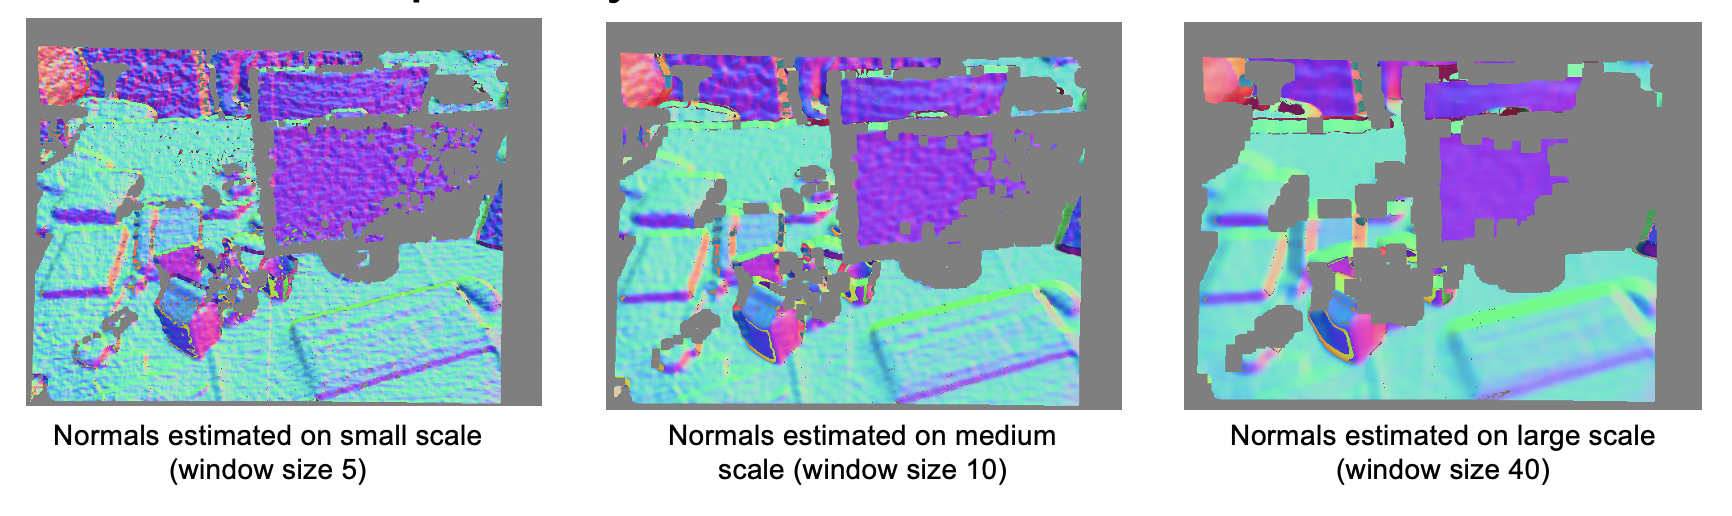
\includegraphics[width=\textwidth]{images/Screen Shot 2020-05-27 at 7.43.01 PM.png}
\label{fig:diff_scales}
\end{figure}

Examples of normals estimated on different scales can be found on figure \ref{fig:diff_scales}.

After obtaining $\left\{I^n_{w_i}\right\}$ we train a fully-convolutional neural network with input shape $\left|W\right| \times H \times W \times 3$ and output shape $H \times W \times 3$. To satisfy requirement \ref{eq:1} we afterwards normalize final normals field $I^n$ along last axis.

\section{Dataset}

Training a neural network requires convenient ground truth. Recently well estimated normals suitable to use as ground truth were not available, for example widely used NUYv2 dataset contained geometrically estimated normals and thus was quite noisy. This problem was addressed by several researchers \cite{matterport, physically-based-rendering}. In our work we use Matterport dataset \cite{matterport}, which contain rich information about indoor environments including multi-view reconstructed meshes and normals. This data has been used extensively since Matterport dataset had been published \cite{deep_surf, deep_depth_compl}; many usages proved that it is quite reliable to be used as ground truth for normal estimation tasks.

\section{Multidimensional integral images} \label{integ-im}

Running multiscale normal estimation algorithm from section \ref{method} would be computationally expensive. For each of scales from $\mathcal{W}$ for each pixel from $I^d$ one has to calculate $4 \times 4$ matrix $C_{i,j,w} = \left[P_{i,j,w}^\top \mathbbm{1}_{w^2} \right]^\top \left[P_{i,j,w}^\top \mathbbm{1}_{w^2} \right]$ and then find SVD of it. Here $P_{i,j,w}$ denotes all points lying inside $w$-sized square window around pixel with coordinates $i$, $j$. Assuming complexity of $4  \times 4$ SVD is constant, resulting complexity of this approach would be 
\[
O\left(\left|\mathcal{W}\right| \times H \times W \times w_{max} ^ 2\right).
\]

To avoid recalculations of matrix $C$ following approach is implemented in our work. We precalculate matrix
\[
X = 
\begin{pmatrix}
\tilde{\bm{d}_{1,1}} \tilde{\bm{d}_{1,1}}^\top & \dots & \tilde{\bm{d}_{1,W}} \tilde{\bm{d}_{1,W}}^\top \\
\vdots & \ddots & \vdots \\
\tilde{\bm{d}_{H,1}} \tilde{\bm{d}_{H,1}}^\top & \dots & \tilde{\bm{d}_{H,W}} \tilde{\bm{d}_{H,W}}^\top \\
\end{pmatrix},
\]
where
\[
\tilde{\bm{d}_{i,j}} = \begin{pmatrix}
I^d_{i,j} \\
1
\end{pmatrix}.
\]

Now $C_{i,j,w}$ can be calculated as follows
\[
C_{i,j,w} = \sum_{k, l \in N_w(i, j)} X[k,l,:,:],
\label{eq:sum}
\]
assuming that $N_w(i, j)$ contains all pixels inside $w$-sized window around pixel $(i, j)$.

Complexity of new approach is 
\[
O\left(H \times W + \left|\mathcal{W}\right| \times H \times W \times w_{max} ^ 2\right).
\]

Complexity did not improve as soon as we replaced matrix multiplication with summation which both have complexity of squared window size $w^2$. However, another trick can be applied to get rid of summation. We create a multidimensional \textit{Integral Image} matrix\footnote{Originally known as \textit{Summed-Area Table} \cite{integral-image}}
\[
S = 
\begin{pmatrix}
0 & 0 & \dots & 0 \\
0 & \sum_{k=1}^1 \sum_{l=1}^1 X[k,l,:,:] & \dots & \sum_{k=1}^1 \sum_{l = 1}^W X[k,l,:,:] \\
\vdots & \vdots & \ddots & \vdots \\
0 & \sum_{k=1}^H \sum_{l=1}^1 X[k,l,:,:] & \dots & \sum_{k=1}^H \sum_{l=1}^W X[k,l,:,:] \\
\end{pmatrix}.
\]

Using $S$ we now can calculate sum of any arbitrary rectangle subarea of $X$ within constant time.
\begin{equation} \label{eq:sum_ii}
\sum_{k=K_1}^{K_2} \sum_{k=L_1}^{L_2} X[k,l] = S[K_2+1, L_2+1] - S[K_1, L_2+1] - S[K_2+1, L_1] + S[K_1, L_1].
\end{equation}

While this idea was originally proposed to work with images, in our work we extend it to work with multidimensional tensors.

By using integral images we can effectively get rid of summation \ref{eq:sum}. Thus, our final complexity is
\[
O\left(H \times W + \left|\mathcal{W}\right| \times H \times W \right) = O\left(\left|\mathcal{W}\right| \times H \times W \right).
\]

Even more performance profit may be achieved if one executes operation \ref{eq:sum_ii} as a convolution over matrix $I$ with $(w + 1) \times (w + 1)$ kernel 
\[
K = 
\begin{pmatrix}
1 & 0 & \dots & 0 & -1 \\
0 & 0 & \dots & 0 & 0 \\
\vdots & \vdots & \ddots & \vdots & \vdots \\
0 & 0 & \dots & 0 & 0 \\
-1 & 0 & \dots & 0 & 1
\end{pmatrix}.
\]

Comparison of different implementation performances can be found in table \ref{table:perf}.

\begin{table}
\centering
\begin{tabular}{ | c | c | c | c | c | }
 \hline
 & Naive implementation & Integral images & Integral images + conv & open3d \\ 
 \hline
 Precalculation & - & 0.5s & 0.5s  & - \\  
 \hline
 Normal estimation & 2s $\times$ 5  & 0.7s $\times$ 5  & 0.2s $\times$ 5 & 1s $\times$ 5 \\  
 \hline
 All & 10s & 4s  & \textbf{1.5s}  & 5s \\
 \hline
\end{tabular}
\caption{Comparison of normal estimation algorithms performances.}
\label{table:perf}
\end{table}